% !TeX encoding=unicode
% !TeX spellcheck = en-US

\chapter{Application examples}
\label{ch:examples}
This chapter presents two examples of application for interpolation grids.
They demonstrate how they extend the number of possible calculations and allow a level of detail in the study of uncertainties that would be very expensive otherwise.
%
\section{PDF uncertainty in cross section calculations}
The application of the interpolation method is sensible every time a calculation has to be repeated plenty of times.
This situation is given for instance, when the uncertainty from a PDF set is meant to be included in a cross section calculation.
Modern PDF sets contain a large number of different samples that can be used to derive the inherent uncertainty.
Having verified that the interpolation grids allow for PDF reweighting in the previous chapter, it is now justified to use them to compute the PDF uncertainty.
Here we consider the NNPDF 3.0 NLO set \cite{nnpdf30}, which consists of \num{101} samples each for \num{5} different values of $\alpha_s$ between \num{0.115} and \num{0.121}.
The grid that has been filled with 100 million events using the central value of the CT10 set is used to calculate a total of 505 replicas for the Higgs $p_\perp$ in \cref{fig:nnpdf_band}.
The similarity between the \appl{} and \fnlo{} plots confirms the correctness of the calculation, as inaccuracies would propagate quite differently in the two implementations.
Once again we see the effects of an insufficient phase space run that have already appeared in \cref{fig:scalesvar_hnlo_appl,fig:pdfvar_hnlo_appl}.
Another thing to observe is that the PDF uncertainty is significantly smaller than the scale uncertainty, even when combined with the error on $\alpha_s$.
The ratio between them is roughly $\frac{1}{6}$.
%
\begin{figure}
	\centering
	\begin{subfigure}[]{0.49\textwidth}
		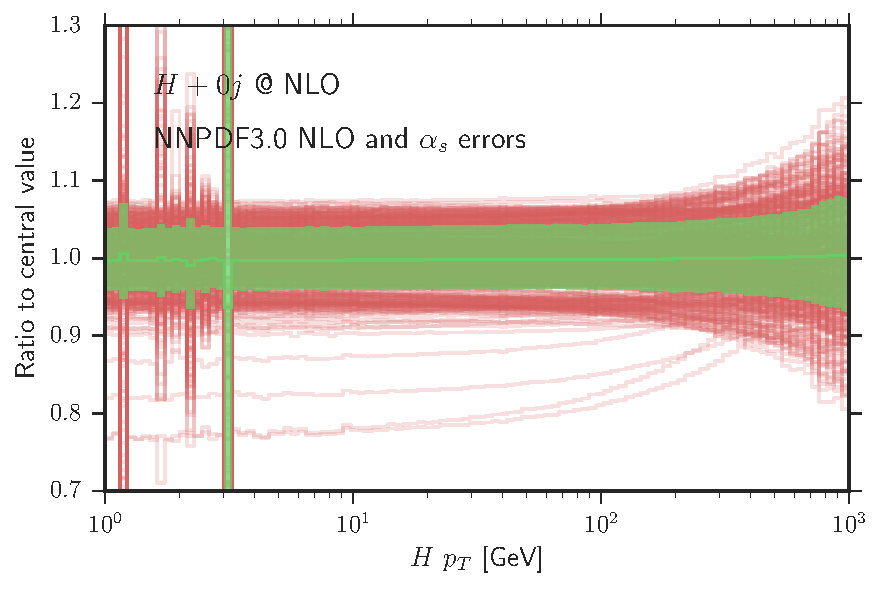
\includegraphics[width=\textwidth]{images/nnpdf_band_appl.pdf}
		\caption{\appl{}}
	\end{subfigure}
	\hfill
	\begin{subfigure}[]{0.49\textwidth}
		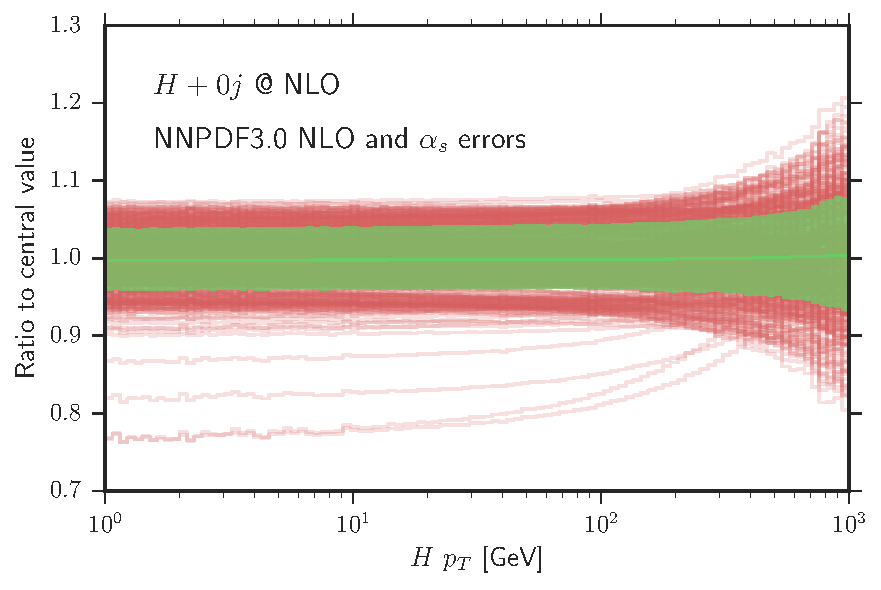
\includegraphics[width=\textwidth]{images/nnpdf_band_fnlo.pdf}
		\caption{\fnlo{}}
	\end{subfigure}
	\caption{Application example of the interpolation method.
				The figure shows the distribution of replicas from the NNPDF3.0 NLO set including the error on $\alpha_s$ for the $p_\perp$ of the Higgs boson in gluon fusion.
				The green area highlights the 1-$\sigma$ confidence interval.}
	\label{fig:nnpdf_band}
\end{figure}
%
\section{Detailed scale dependence of the cross section}
When one wishes to estimate the uncertainty of a fixed order calculation, a common method is to vary the renormalization and factorization scales simultaneously or independently by some factor, usually a factor of 2.
This way one hopes to get a reasonable estimate of the corrections due to higher order terms.
Typically, only the boundary values are calculated because of limited resources.
However, using interpolation grids, any combination of scale factors can be evaluated very fast.
To demonstrate this, \cref{fig:3dscale} shows the total cross section of inclusive Higgs production through gluon fusion for different combinations of scale factors, calculated using a \fnlo{} grid.
Both the renormalization scale and the factorization scale are independently varied by 13 factors between $\frac{1}{4}$ and \num{4} resulting in a total number of 169 calculations of the cross section.
We see that the dependence on the factorization scale is low whereas we observe a strong dependence on the renormalization scale.
%
\begin{figure}
	\centering
	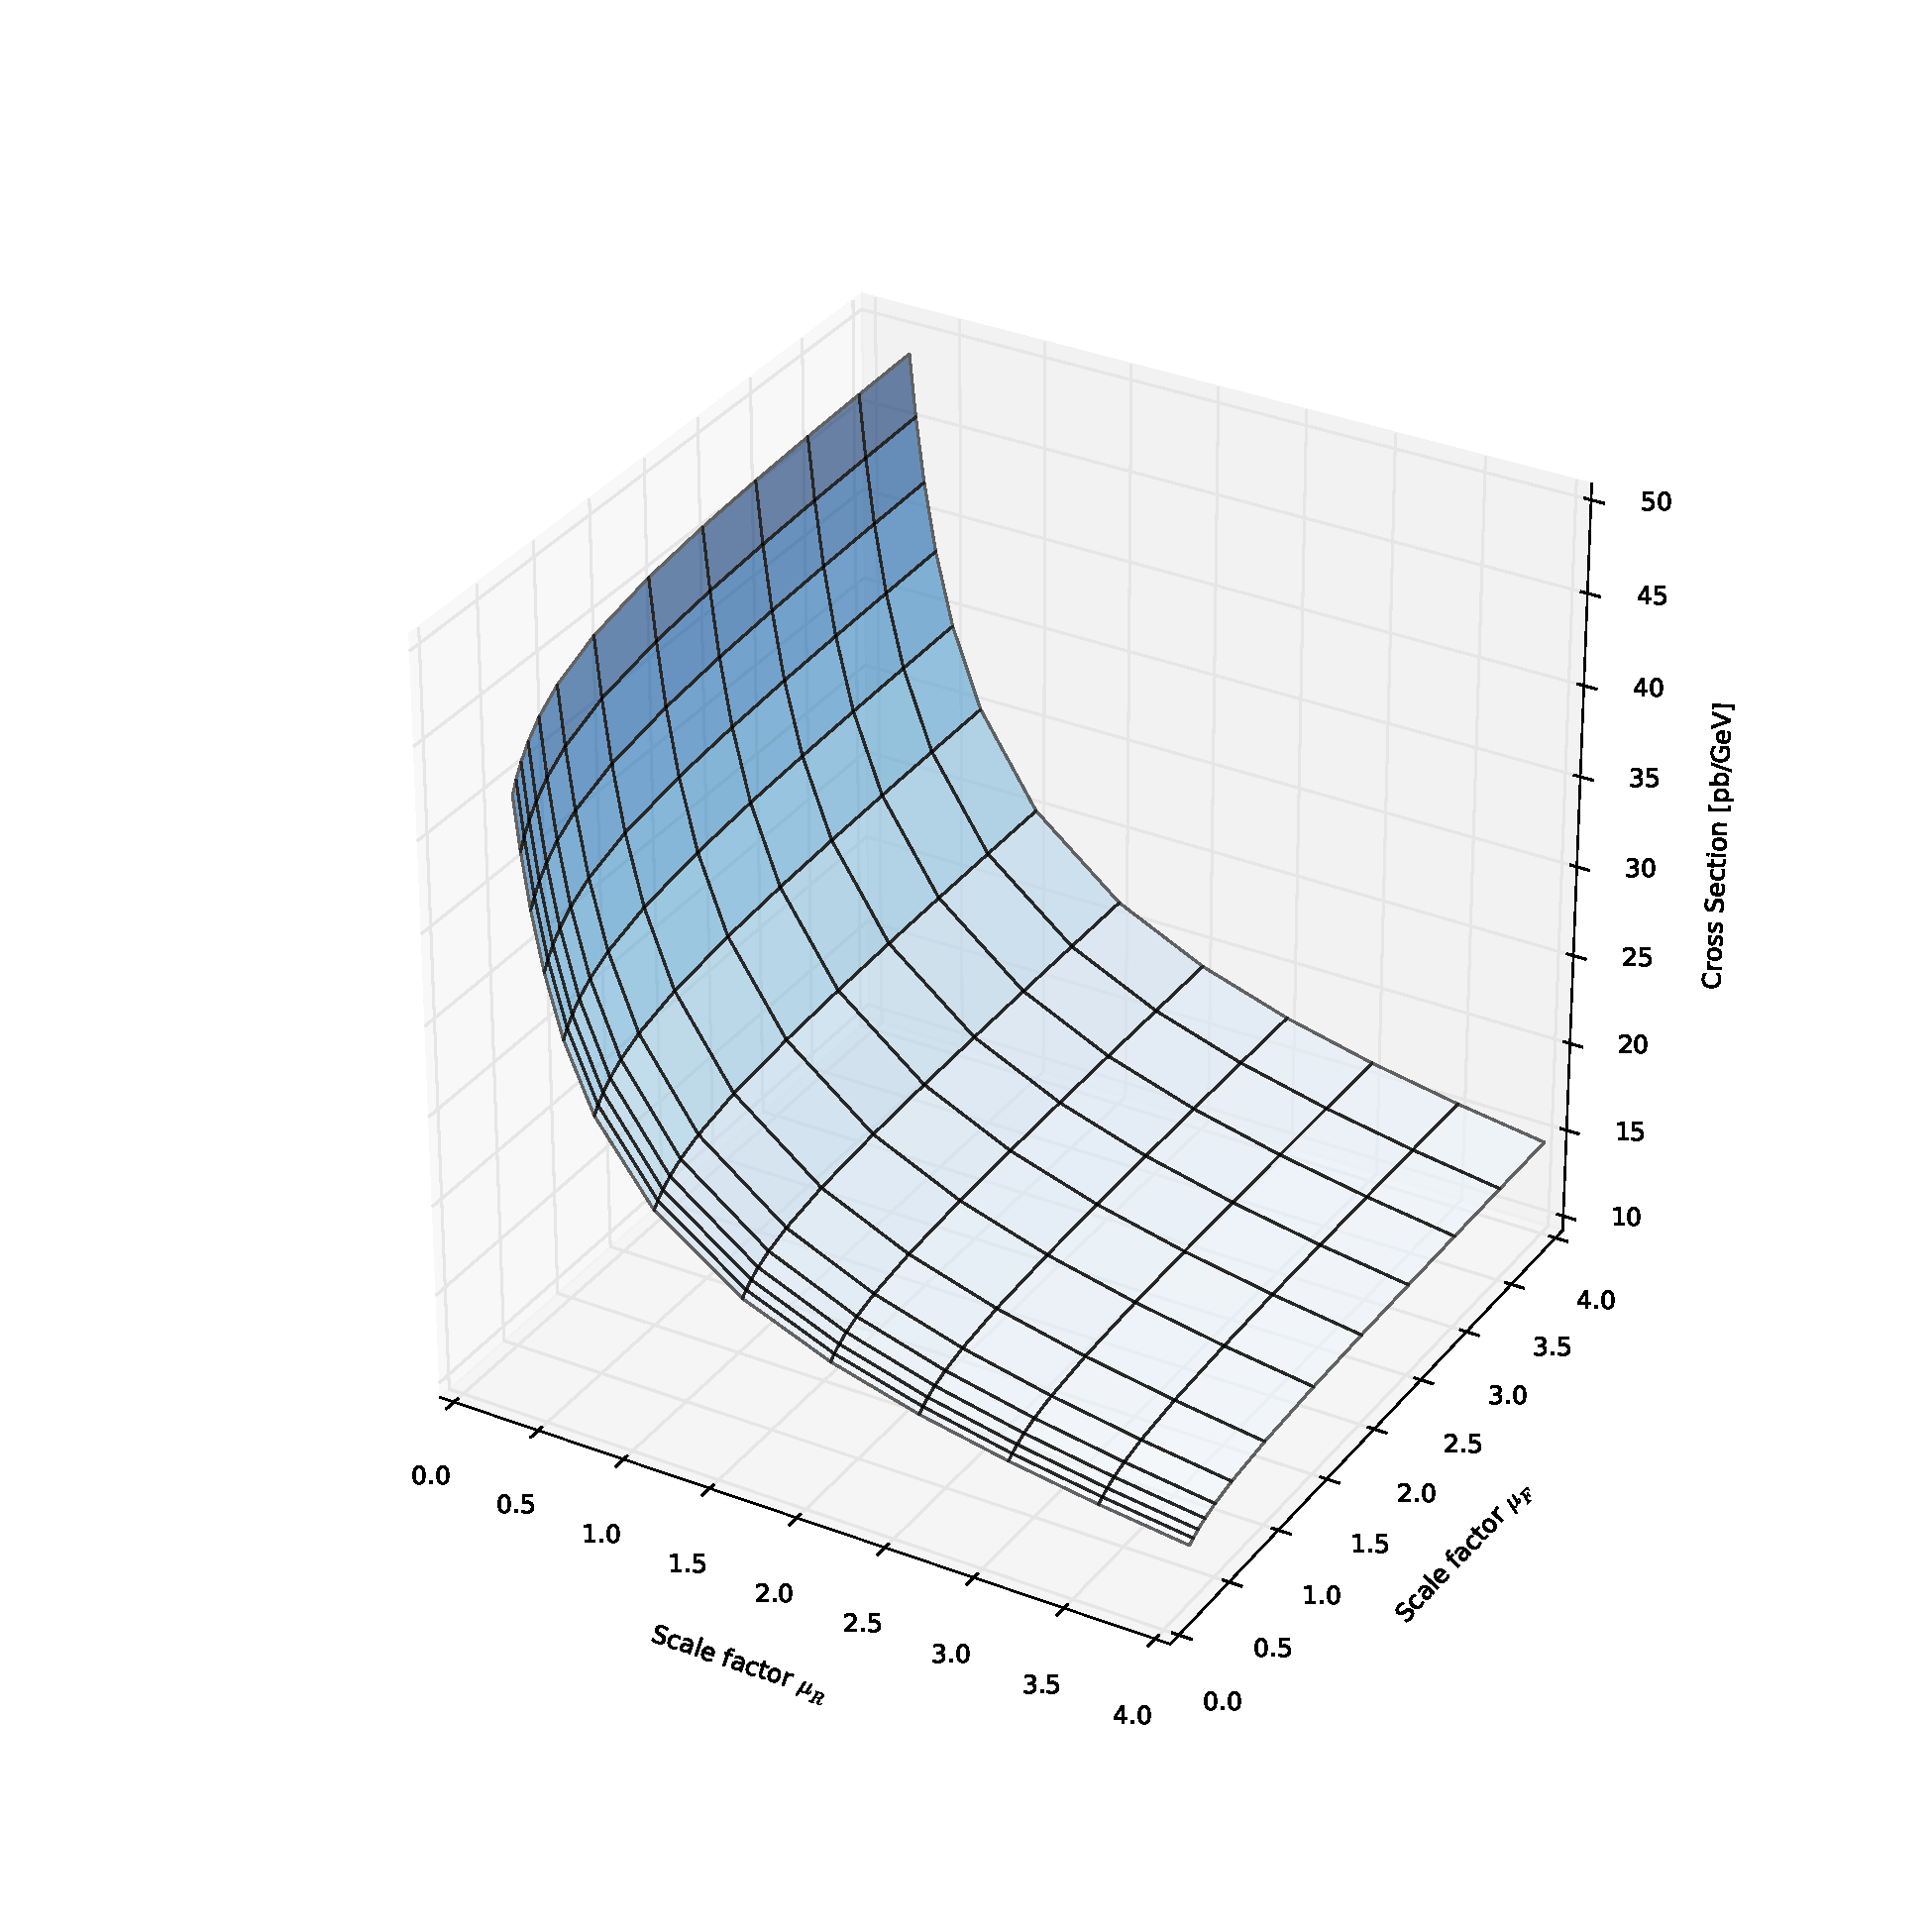
\includegraphics[width=0.8\textwidth]{images/3dscale.pdf}
	\caption{Application example of the interpolation method.
			The figure shows the total cross section of inclusive Higgs production at NLO as a function of the renormalization and factorization scales.
			The values have been generated from a \fnlo{} grid.}
	\label{fig:3dscale}
\end{figure}
%

Calculations such as this one and the example illustrated before would be extremely costly if done explicitly.
If they are time-critical, explicit calculations become impossible.
Interpolation tools offer much more flexibility in these cases.
Especially the estimation of uncertainties can be much more differentiated.
